\documentclass[11pt,a4paper]{article}
\usepackage{tikz}
\usetikzlibrary{arrows.meta,positioning}
\usepackage{tabularx}
\usepackage{amsmath,amssymb,amsthm}
\usepackage{geometry}
\geometry{margin=1in}
\usepackage{hyperref}
\usepackage{graphicx}
\usepackage{setspace}
\onehalfspacing

\title{\textbf{Paper A-14: Earth Volcanology:\\ A Constraint-Driven Flux Dynamics (CDFD) Perspective}}
\author{Steve Bico Mujjabi, MD\\
\small Independent Researcher\\
\small Founder, Vura Labs\\
\small Kampala, Uganda\\
\small ORCID: 0009-0001-0556-5516}
\date{May 2026}

\begin{document}
\maketitle


\begin{abstract}
This paper develops a falsifiable CDFD/AFL model of Earth Volcanology. It maps magma buoyancy, volatile pressure, heat, and tectonic forcing to driving flux $\Phi$, conduit geometry, rock strength, crystallization, and degassing limits to active constraint $C$, deformation, fracture, vent opening, convection, and pressure release to responsiveness $S$, and chamber recharge, crystal mush, conduit scars, and edifice history to structural memory $M_s$. The target outcome is unrest, eruption style, magnitude, and recovery, tested against seismicity, deformation, gas, petrology, thermal imagery, and eruption chronologies. The paper treats universality as a shared model architecture rather than an assertion that unlike systems have the same material mechanism. It states the negative result that would make the mapping unnecessary and places the domain claim inside the cumulative CDFD programme and its reproducible runtime boundary.
\end{abstract}

\section*{Symbol Conventions}

\noindent\textbf{CDFD/AFL Part IV symbol convention.}
\begin{center}
{\small
\begin{tabular}{p{0.15\linewidth}p{0.34\linewidth}p{0.41\linewidth}}
\hline
Symbol & Part IV meaning & Cross-domain reading \\
\hline
$\Phi$ & Driving flux or throughput & Energy, matter, signal, capital, information, traffic, force, or biological load entering a system \\
$C$ & Active constraint or capacity burden & Bottleneck, resistance, boundary, scarcity, toxicity, regulation, topology, latency, or load-bearing limit \\
$S$ & Responsiveness or adaptive surface & The system's ability to reconfigure, buffer, route, repair, learn, or preserve function under changing load \\
$M_s$ & Structural memory & Stored damage, hysteresis, inherited topology, institutional memory, trained weights, ecological legacy, or retained state \\
$\Psi_s$ & Adaptive operating ratio $(\Phi/C)\cdot S\cdot M_s$ & Local bookkeeping gauge for constrained operation, overload, recovery, or regime change; not a universal constant \\
$\Lambda$ & Life Number or capstone surplus ratio where explicitly defined & Reserved for Part II-derived life-number notation or synthesis-level surplus measures, never an undefined decoration \\
\hline
\end{tabular}
}
\end{center}

\noindent\textbf{Greek-symbol convention.}
\begin{center}
{\small
\begin{tabular}{p{0.15\linewidth}p{0.34\linewidth}p{0.41\linewidth}}
\hline
Symbol & Local role & Interpretation rule \\
\hline
$\alpha$ & Accumulation or reinforcement coefficient & Sets how fast a pathway, constraint, habit, cascade, or retained structure grows under load \\
$\beta$ & Relaxation, decay, clearance, or washout coefficient & Sets loss, recovery, damping, forgetting, degradation, or return toward baseline \\
$\gamma$ & Coupling, diffusion, redistribution, or transfer coefficient & Sets spread across nodes, layers, tissues, markets, infrastructures, media, or physical phases \\
$\delta,\epsilon$ & Perturbation, tolerance, small offset, or numerical guard & Used only as local thresholds, stability margins, measurement tolerances, or stress increments \\
$\eta,\lambda,\mu,\nu$ & Efficiency, rate, baseline, intensity, or frequency terms & Meaning is fixed by the equation, subscript, and domain-specific proxy in the paragraph where the term appears \\
$\rho,\sigma,\tau,\phi$ & Density/correlation, variability/noise, time-scale, phase, or field terms & Local coefficients only; subscripts bind them to the named pathway, domain, or experiment \\
$\Omega,\Lambda$ & Domain/state space; Life Number where defined & $\Omega$ names a modeled state space; $\Lambda$ carries life-number or synthesis notation only when the paper defines it \\
\hline
\end{tabular}
}
\end{center}

\section{Series Context}

Part I sets the flow--constraint language used here \cite{MujjabiPartI2026}. Part II develops the Life Number and the origins-of-life use of the same notation \cite{MujjabiPartII2026}. Part III applies AFL to biology and medicine \cite{MujjabiPartIII2026}. Part IV \cite{MujjabiPartIV2026}, DOI \url{https://doi.org/10.5281/zenodo.20395901}, is the cross-domain stress test: it asks where the notation clarifies measurement, and where it becomes only a metaphor.

\section{Introduction}

\subsection{The Mujjabi Universal Capacity Law}
Building directly upon the Fundamental Physics (Part I) \cite{MujjabiPartI2026}, the \textbf{Mujjabi Universal Capacity Law} proposes that across all scales---from black hole event horizons to global financial markets and power grids---driving high flux ($\Phi$) against a rigid topological constraint ($C$) can drive system saturation. When $\Phi/C$ approaches critical thresholds, the system does not scale linearly; it undergoes a topological phase transition.

\subsection{The Mujjabi Universal Memory Law}
The \textbf{Mujjabi Universal Memory Law} frames persistent systemic collapse. When a complex network fails to clear its structural memory ($M_s$) and its relaxation parameter decays ($\tau_{relax} \to \infty$), temporary stressors become permanent rigidities. This is the proposed CDFD mechanism behind ecological death, economic depressions, and infrastructural gridlock.

Magma generation deep in the Earth's mantle creates buoyant, low-density melts that ascend toward the surface. During this ascent, pressure decreases, allowing dissolved volatiles (such as $H_2O$ and $CO_2$) to exsolve and form bubbles. The dynamics of these bubbles, and the structural integrity of the surrounding rock, dictate whether a volcano will gently erupt lava or explosively detonate.

Applying CDFD to volcanology reveals that a volcano is functionally a high-pressure nozzle attempting to regulate thermodynamic throughput.

\section{The Magmatic Conduit as an Adaptive Surface}
We define the thermodynamic state of the magma chamber and conduit using the Universal Adaptive Ratio:
\begin{equation}
    \Psi_s = \left( \frac{\Phi}{C} \right) \cdot S \cdot M_s
\end{equation}

In volcanic systems:
\begin{itemize}
    \item \textbf{Flux ($\Phi$)}: The upward flow of magma and, critically, the volumetric expansion flux of exsolving gases.
    \item \textbf{Constraint ($C$)}: Lithostatic confining pressure, magma viscosity, and the structural rigidity of the vent caprock.
    \item \textbf{Responsiveness ($S$)}: The elasticity of the magma chamber walls and the ability of the magma to deform (low viscosity).
    \item \textbf{Memory ($M_s$)}: Crystallization and cooling. As magma stalls, it cools and crystallizes, increasing its viscosity and forming a solid plug. This physical state locks the system's memory, severely cementing the constraint.
\end{itemize}

\subsection{Effusive vs. Explosive Eruptions}
In a basaltic shield volcano (like those in Hawaii), the magma has low viscosity. The constraint $C$ remains low, and the system can continuously process the upward flux $\Phi$ smoothly. The system remains near $\Psi_s \approx 1$. The eruption is effusive and constant.

Conversely, in a stratovolcano with highly viscous, silica-rich magma, the system behaves pathologically. As gases exsolve ($\Phi$ spikes), the high viscosity prevents the bubbles from escaping. The magma cools, crystallizing into a solid plug at the vent (high $M_s$). The constraint $C$ becomes absolute.

The system enters a chronic choke state ($\Psi_s \ll 1$). The upward flux from the mantle continues to compress into the chamber. Because the constraint $C$ cannot flex, the internal pressure exceeds the fracture strength of the rock. The constraint fails catastrophically, dropping $C$ to zero in an instant. The pressurized gas expands supersonically, resulting in a Plinian explosive eruption that atomizes the magma into ash.



\section{Measurement Layer}

The first job in any domain is to choose proxies before drawing conclusions. $\Phi$ may be a rate of material, energy, information, capital, or signal flow. $C$ is the bottleneck that slows or redirects that flow. $S$ measures the system's ability to reconfigure under stress, and $M_s$ records the past load that still changes present behavior. A useful application gives those four terms observable definitions, a time scale, and a failure condition. If a standard domain model explains the same data more cleanly, the CDFD/AFL mapping should give way.

\subsection{Current Runtime Diagnostic: Universal Network Cascade}
The release-local discovery script keeps this paper tied to the current CDFD Runtime \cite{CDFDRuntime2026}, including RK4 field updates, surface dynamics, structural-memory diffusion, and a finite-value audit. In the 2026-06-04 runtime pass, the localized hub-drive stress test ended with hub $\Psi_s=5.21$, peak network $\Psi_s=5.21$, 21 nodes above $\Psi_s>1.5$, and 37 maximum memory-locked nodes. I treat those numbers as a runtime sanity check and as a target for later domain measurement, not as a substitute for field data.


% BEGIN PART IV MAJOR UNIVERSAL UPGRADE
\section{Major Universal Upgrade: Mechanism, Scale, and Tests}

\subsection{Observable Translation}

The paper-specific translation begins with an observable chain rather than a
verbal analogy. For Earth Volcanology, the proposed drive is magma buoyancy, volatile pressure, heat, and tectonic forcing.
The active limitation is conduit geometry, rock strength, crystallization, and degassing limits. Responsiveness is carried by
deformation, fracture, vent opening, convection, and pressure release, while retained state is represented by
chamber recharge, crystal mush, conduit scars, and edifice history. The outcome to explain is unrest, eruption style, magnitude, and recovery.

\begin{table}[htbp]
\centering
\small
\caption{Operational CDFD/AFL map for Paper A-14.}
\begin{tabularx}{\textwidth}{|l|X|X|}
\hline
\textbf{Term} & \textbf{Paper-specific observable meaning} & \textbf{Measurement question} \\
\hline
$\Phi$ & magma buoyancy, volatile pressure, heat, and tectonic forcing & What rate, load, gradient, or demand enters the focal system? \\
\hline
$C$ & conduit geometry, rock strength, crystallization, and degassing limits & Which measured bottleneck limits transfer, function, or recovery? \\
\hline
$S$ & deformation, fracture, vent opening, convection, and pressure release & Which process changes effective capacity or reroutes the load? \\
\hline
$M_s$ & chamber recharge, crystal mush, conduit scars, and edifice history & Which retained state makes equal present loads produce different futures? \\
\hline
$Y$ & unrest, eruption style, magnitude, and recovery & Which outcome is predicted out of sample, with uncertainty? \\
\hline
\end{tabularx}
\end{table}

\begin{figure}[htbp]
\centering
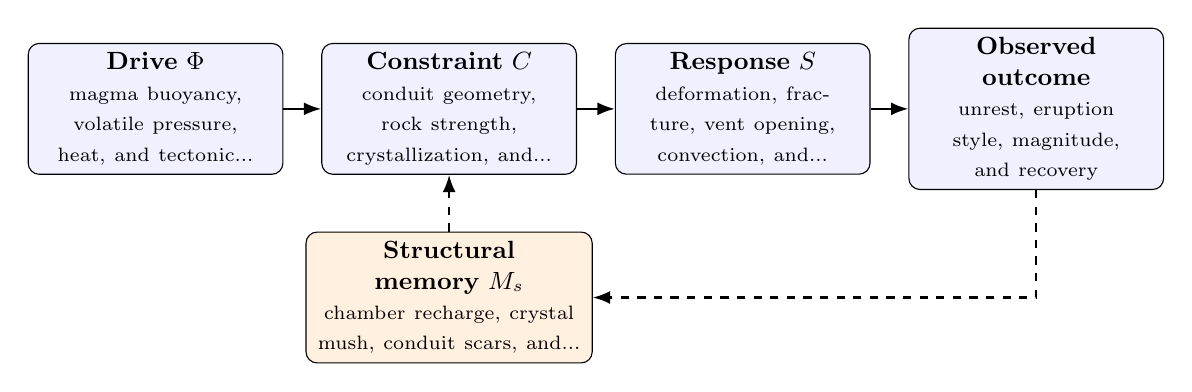
\begin{tikzpicture}[
    node distance=0.48cm,
    every node/.style={font=\small},
    box/.style={draw, rounded corners, align=center, minimum height=1.45cm, text width=3.0cm, fill=blue!6},
    memory/.style={draw, rounded corners, align=center, minimum height=1.25cm, text width=3.4cm, fill=orange!12},
    flow/.style={-{Latex[length=2.2mm]}, thick},
    feedback/.style={-{Latex[length=2.2mm]}, thick, dashed}
]
\node[box] (drive) {\textbf{Drive $\Phi$}\\\scriptsize magma buoyancy, volatile pressure, heat, and tectonic...};
\node[box, right=of drive] (constraint) {\textbf{Constraint $C$}\\\scriptsize conduit geometry, rock strength, crystallization, and...};
\node[box, right=of constraint] (response) {\textbf{Response $S$}\\\scriptsize deformation, fracture, vent opening, convection, and...};
\node[box, right=of response] (outcome) {\textbf{Observed outcome}\\\scriptsize unrest, eruption style, magnitude, and recovery};
\node[memory, below=0.72cm of constraint] (memory) {\textbf{Structural memory $M_s$}\\\scriptsize chamber recharge, crystal mush, conduit scars, and...};
\draw[flow] (drive) -- (constraint);
\draw[flow] (constraint) -- (response);
\draw[flow] (response) -- (outcome);
\draw[feedback] (outcome.south) |- (memory.east);
\draw[feedback] (memory.north) -- (constraint.south);
\end{tikzpicture}
\caption{Paper A-14 observable CDFD/AFL architecture for Earth Volcanology. Solid arrows give the proposed forward chain; dashed arrows make history-dependent feedback explicit.}
\label{fig:a14-architecture}
\end{figure}

\subsection{Minimal Coupled Model}

A paper-level model must separate throughput, constraint accumulation, response,
and history. One deliberately minimal form is
\begin{align}
Y(t) &= \frac{\Phi(t)S(t)}{\epsilon + C(t)}, \\
\frac{dC}{dt} &= \alpha \Phi(t) - \beta S(t)C(t) + \gamma \mathcal{L}C(t), \\
\frac{dM_s}{dt} &= \eta C(t) - \mu M_s(t), \\
\Psi_s(t) &= \frac{\widehat{\Phi}(t)}{\epsilon+\widehat{C}(t)}\,
             \widehat{S}(t)\,[1+\omega\widehat{M_s}(t)] .
\end{align}
Here $Y$ is the measured output, $\epsilon>0$ prevents a singular denominator,
$\mathcal{L}$ is a spatial or network coupling operator, and hats denote
explicitly normalized variables. The sign and magnitude of $\omega$ must be
estimated: memory can preserve useful organization or amplify damage. No fixed
threshold is universal before the variables, normalization, and observation
scale are declared.

For this paper, the hypothesized causal sequence is specific. A change in
magma buoyancy, volatile pressure, heat, and tectonic forcing arrives faster than deformation, fracture, vent opening, convection, and pressure release can compensate.
This raises or redistributes conduit geometry, rock strength, crystallization, and degassing limits. If the load persists,
the retained state encoded by chamber recharge, crystal mush, conduit scars, and edifice history changes the next response, so a later event of equal
magnitude can produce a different trajectory in unrest, eruption style, magnitude, and recovery. The
scientific task is to estimate that sequence against the best ordinary model of
the domain, not merely to redescribe the outcome after it occurs.

\subsection{Cross-Scale Universality Without Mechanistic Erasure}

For the Earth systems family, the universal comparison is between coupled transport, finite environmental capacity, buffering, and retained landscape or ecosystem state. Universality here cannot erase conservation laws, geometry, or scale; it must expose where those domain equations create comparable overload and recovery structures. \cite{Holling1973,Turing1952,BakTangWiesenfeld1987}
The CDFD programme is cumulative: Part I supplies the flow--constraint
foundation \cite{MujjabiPartI2026}; Part II asks when maintained throughput
supports persistent organized states \cite{MujjabiPartII2026}; Part III
develops adaptive limitation and biological memory \cite{MujjabiPartIII2026};
and Part IV \cite{MujjabiPartIV2026} tests how much of that architecture
survives translation. The CDFD Runtime \cite{CDFDRuntime2026} supplies a
reproducible numerical stress surface, but it does not substitute for the
domain evidence named here.

The required scale declaration for this paper is seconds to millennia; bubbles and conduits to volcanic arcs. At short
scales, the key question is whether the incoming drive is transmitted,
buffered, or diverted. At intermediate scales, response changes effective
capacity and network exposure. At long scales, retained structure can alter the
state space itself. A result is genuinely cross-scale only when the aggregation
rule is stated and the same conclusion is not an artifact of averaging.

\subsection{Evidence Ladder and Discriminating Tests}

\begin{table}[htbp]
\centering
\small
\caption{Evidence ladder for Paper A-14. Each rung can fail independently.}
\begin{tabularx}{\textwidth}{|p{0.17\textwidth}|X|X|}
\hline
\textbf{Test} & \textbf{Design} & \textbf{Discriminating result} \\
\hline
Proxy audit & Measure seismicity, deformation, gas, petrology, thermal imagery, and eruption chronologies and preregister how each record maps to $\Phi$, $C$, $S$, $M_s$, and $Y$. & The mapping fails if proxies are non-identifiable, circular, or change meaning across cases. \\
\hline
Load ramp & Apply or observe a recharge pulse into systems with contrasting histories while estimating the dominant constraint and response time. & A threshold claim requires a reproducible nonlinear change and uncertainty bounds, not a visually chosen breakpoint. \\
\hline
Recovery and memory & Match present load across units with different histories, then compare recovery paths. & The memory claim requires history-dependent divergence after current conditions are controlled. \\
\hline
Model comparison & Compare the baseline domain model with and without the CDFD/AFL state variables using held-out data. & The paper's stated falsifier is: history-sensitive variables do not improve eruption-style or unrest interpretation. \\
\hline
\end{tabularx}
\end{table}

The strongest practical design combines a prospective perturbation with a
recovery window. The load-ramp phase estimates where constraint begins to rise
faster than output. The recovery phase estimates $\beta$ and $\mu$, separating
fast relaxation from persistent memory. A topology or coupling intervention
then asks whether rerouting changes the cascade as predicted. Null results are
informative because they identify domains in which the universal notation adds
no measurable value.

\subsection{Research Programme and Boundary Conditions}

The immediate research programme has four steps. First, construct a documented
dataset from seismicity, deformation, gas, petrology, thermal imagery, and eruption chronologies and retain raw units before normalization.
Second, fit a baseline domain model and report its calibration and out-of-sample
error. Third, add the smallest identifiable CDFD/AFL state extension and test
whether it improves prediction of unrest, eruption style, magnitude, and recovery. Fourth, repeat the
analysis across the declared scale range and publish negative cases as part of
the universality audit.

Three boundaries are non-negotiable. Correlation between flow and failure does
not identify a constraint mechanism. A fitted memory term does not prove that
the stored state has the same material meaning in another domain. Finally, a
runtime cascade is evidence about the implementation, not evidence that the
real system follows it. The paper becomes stronger when it can say precisely
where the translation stops.


% END PART IV MAJOR UNIVERSAL UPGRADE

\section{Conclusion}
Volcanic eruptions are thermodynamic venting mechanisms. By applying the CDFD equation, we see that effusive eruptions represent a healthy, regulated flow regime, while explosive eruptions represent the catastrophic failure of an over-constrained system locked by magmatic memory. The Earth regulates its internal heat flux using a comparable flow--constraint architecture that a biological cell uses to regulate its metabolic gradients.
\section*{Conflict of Interest} The author declares no conflict of interest.
\section*{Data Availability}
Part-specific runtime diagnostics are under each Part's \path{outputs/} directory.

Release-wide code: \path{Part_E_Synthesis/supplementary/}.

Generated summaries: \path{Part_E_Synthesis/outputs/}.

Figures: \path{Part_E_Synthesis/figures/}.


\section{Reference Layer}
\bibliographystyle{plain}
\bibliography{universal_afl_references}
\end{document}
